% !TeX spellcheck = it_IT
\title{Informatica Teorica}
\author{Massimo Perego}
\date{}

\documentclass[11pt]{report}
\usepackage{graphicx} 
\usepackage{amsmath}
\usepackage{amssymb}
\usepackage{amsfonts}
\usepackage[hidelinks]{hyperref}
\usepackage[autostyle, english = american]{csquotes}
\usepackage[parfill]{parskip}
\MakeOuterQuote{"}

\usepackage{./commands}

\usepackage{dutchcal}
\usepackage{tikz}
\usetikzlibrary{shapes,arrows,positioning, intersections, calc}
\usepackage{amsthm}
\usepackage{array}
\usepackage{calc}
\newcolumntype{C}[1]{wc{\widthof{#1}}} % fixed width & centered
\usepackage{ifthen}
\usepackage{stmaryrd}
\usepackage{multirow}
\usepackage{mathtools}
\usepackage[italiano,noline]{algorithm2e}
\usepackage{tcolorbox}
\usepackage{setspace}

\makeatletter
\renewcommand{\@chapapp}{Capitolo}
\renewcommand{\contentsname}{Indice}
\makeatother

\begin{document}
	
	\tikzstyle{block} = [draw, rectangle, minimum height=2em, minimum width=3em]
	
	\maketitle
	\tableofcontents
	\newpage
	
	% !TeX spellcheck = it_IT
% !TeX root = ../it.tex

\chapter*{Introduzione}
\addcontentsline{toc}{chapter}{Introduzione}

Si "contrappone" all'informatica applicata, ovvero qualsiasi applicazione dell'informatica atta a raggiunger uno scopo, dove l'informatica è solamente lo strumento per raggiungere in maniera efficace un obiettivo.\\
Con "\textit{informatica teorica}" l'oggetto è l'informatica stessa, si studiano i fondamenti della disciplina in modo rigoroso e scientifico. Può essere fatto ponendosi delle questioni fondamentali: il \textit{cosa} e il \textit{come} dell'informatica, ovvero cosa è in grado di fare l'informatica e come è in grado di farlo.

\paragraph{Cosa:} L'informatica è "la disciplina che studia l'informazione e la sua elaborazione automatica", quindi l'oggetto sono l'informazione e i dispositivi di calcolo per gestirla; scienza dell'informazione. Diventa lo studio come risolvere automaticamente un problema. Ma tutti i problemi sono risolvibili in maniera automatica? Cosa è in grado di fare l'informatica? \\

La branca dell'informatica teorica che studia cosa è risolvibile si chiama \textbf{Teoria della Calcolabilità}, studia cosa è calcolabile per via automatica. Spoiler: non tutti i problemi sono risolvibili per via automatica, e non potranno mai esserlo per limiti dell'informatica stessa. Cerchiamo una caratterizzazione generale di cosa è calcolabile e cosa no, si vogliono fornire strumenti per capire ciò che è calcolabile. La caratterizzazione deve essere fatta matematicamente, in quanto il rigore e la tecnica matematica permettono di trarre conclusioni sull'informatica.

\paragraph{Come:} Una volta individuati i problemi calcolabili, come possiamo calcolarli? Il dominio della \textbf{Teoria della Complessità} vuole descrivere le risoluzione dei problemi tramite mezzi automatici in termini di risorse computazionali necessarie. Una "risorsa computazionale" è qualsiasi cosa che viene consumata durante l'esecuzione per risolvere il problema, come possono essere elettricità o numero di processori, generalmente i parametri più importanti considerati sono tempo e spazio di memoria. Bisognerà definire in modo preciso cosa si intende con "tempo" e "spazio". Una volta fissati i parametri bisogna definire anche cosa si intende con "risolvere efficientemente" un problema, in termini di tempo e spazio.\\

La teoria della calcolabilità dice quali problemi sono calcolabili, la teoria della complessità dice, all'interno dei problemi calcolabili, quali sono risolvibili efficientemente.\\
	
	% !TeX spellcheck = it_IT
% !TeX root = ../it.tex

\chapter{Teoria della Calcolabilità}

\section{Notazione}

\subsection{Funzioni}

\paragraph{Funzione:} Una funzione $f$ dall'insieme $A$ all'insieme $B$ è una legge che dice come associare a ogni elemento di $A$ un elemento di $B$. Si scrive
$$ f: A \rightarrow B $$
E chiamiamo $A$ dominio e $B$ codominio. Per dire come agisce su un elemento si usa $f(a) = b$, $b$ è l'immagine di $a$ secondo $f$ (di conseguenza $a$ è la controimmagine).\\
Per definizione di funzione, è possibile che elementi del codominio siano raggiungibili da più elementi del dominio, ma non il contrario. Possiamo classificare le funzioni in base a questa caratteristica:
\begin{itemize}
	\item \textbf{Iniettiva:} $f: A \rightarrow B$ è iniettiva sse $\forall a,b \in A$, $a \neq b \implies f(a) \neq f(b)$
	\item \textbf{Suriettiva:} $f: A \rightarrow B$ è suriettiva sse $\forall b \in B$, $\exists a \in A: f(a) = b$: un altro modo per definirla è tramite l'insieme immagine di $f$, definito come
	$$ \ImSet_f = \{b \in B: \exists a, f(a) = b \} = \{f(a): a \in A \} $$
	Solitamente $\text{Im}_f \subseteq B$, ma $f$ è suriettiva sse $ \ImSet_f = B$;
	\item \textbf{Biettiva:} $f: A \rightarrow B$ è biettiva sse è sia iniettiva che suriettiva, ovvero
	$$
	\begin{array}{c l}
		\forall a, b \in A, a \neq b: & f(a) \neq f(b) \\
		\forall b \in B, \exists a \in A: & f(a) = b
	\end{array}
	\implies \forall b \in B, \exists! a \in A: f(a) = b
	$$
\end{itemize}

\paragraph{Inversa:} Per le funzioni biettive si può naturalmente associare il concetto di "inversa": dato $f: A \rightarrow B$ biettiva, si definisce inversa la funzione $f^{-1}: B \rightarrow A$ tale che $f^{-1} (b) = a \Leftrightarrow f(a) = b$.\\

\paragraph{Composizione di funzioni:} Date $f: A \rightarrow B$ e $g: B \rightarrow C$, $f$ composto $g$ è la funzione $g \circ f: A \rightarrow C$ definita come $g \circ f(a) = g(f(a))$. Generalmente non commutativo, $f \circ g \neq g \circ f$, ma è associativo.\\

\paragraph{Funzione identità:} Dato l'insieme $A$, la funzione identità su $A$ è la funzione $i_A: A \rightarrow A$ tale che $i_A (a) = a$, $\forall a \in A$.\\

Un'altra possibile definizione per l'inversa diventa:
$$ f^{-1} \circ f = i_A \wedge f \circ f^{-1} = i_B $$

\paragraph{Funzioni Parziali:} Se una funzione $f: A \rightarrow B$ è definita per $a \in A$ si indica con $f(a) \downarrow$ e da questo proviene la categorizzazione: una funzione è \textbf{totale} se definita $\forall a \in A$, \textbf{parziale} altrimenti (definita solo per qualche elemento di $A$).\\

\paragraph{Insieme Dominio:} Chiamiamo \textbf{dominio} (o campo di esistenza) di $f$ l'insieme
$$ \Dom_f = \left\{a \in A | f(a) \downarrow \right\} \subseteq A $$
Quindi se $\Dom_f = A$ la funzione è totale, se $\Dom_f \subsetneq A$ allora è una funzione parziale.\\

\paragraph{Totalizzazione:} Si può \textbf{totalizzare una funzione parziale} $f$ definendo una funzione a tratti $\overline{f}: A \rightarrow B \cup \{\bot\}$ tale che
$$ 
\overline{f} (a) = \begin{cases}
	f(a) & a \in \Dom_f(a) \\
	\bot & \text{altrimenti}
\end{cases}
$$
Dove $\bot$ è il \textbf{simbolo di indefinito}, per tutti i valori per cui la funzione di partenza $f$ non è definita. Da qui in poi $B_\bot$ significa $B \cup \{\bot\}$.\\

\paragraph{Insieme delle funzioni:} L'insieme di tutte le funzioni che vanno da $A$ a $B$ si denota con
$$ B^A = \{f: A \rightarrow B \} $$
La notazione viene usata in quanto la cardinalità di $B^A$ è esattamente $|B|^{|A|}$, con $A$ e $B$ insiemi finiti.\\
Volendo includere anche tutte le funzioni parziali: 
$$ B^A_\bot = \{f: A \rightarrow B_\bot \} $$
Le due definizioni coincidono, $B^A = B^A_\bot$, ma quest'ultima permette di mettere in evidenza che tutte le funzioni presenti sono totali o totalizzate.\\ 

\subsection{Prodotto Cartesiano}

Chiamiamo \textbf{prodotto cartesiano} l'insieme 
$$ A \times B = \{(a,b) | a \in A \wedge b \in B \} $$
Rappresenta l'insieme di tutte le coppie ordinate di valori in $A$ e $B$. In generale non è commutativo, a meno che $A=B$.\\

Può essere esteso a $n$-uple di valori:
$$ A_1 \times \dots \times A_n = \{(a_1, \dots, a_n) | a_i \in A_i\} $$
Il prodotto di $n$ volte lo stesso insieme verrà, per comodità, indicato come
$$ A \times \dots \times A = A^n $$

\paragraph{Proiettore:} Operazione "opposta", il proiettore $i$-esimo è una funzione che estrae l'$i$-esimo elemento di una tupla, quindi è una funzione
$$ \pi_i: A_1 \times \dots \times A_n \rightarrow A_i \tc \pi_i (a_1, \dots, a_n) = a_i $$
La proiezione sull'asse in cui sono presenti i valori dell'insieme $a_i$.\\

\subsection{Funzione di Valutazione}
Dati $A,B$ e $B^A_\bot$ si definisce \textbf{funzione di valutazione} la funzione
$$ \omega: \bat \times A \rightarrow B \tc \omega (f,a) = f(a) $$
Prende una funzione $f$ e la valuta su un elemento $a$ del dominio. Si possono fare due tipi di analisi su questa funzione: 
\begin{itemize}
	\item Fisso $a$ e provo tutte le $f$, ottenendo un \textit{benchmark} di tutte le funzioni su $a$
	\item Fisso $f$ e provo tutte le $a$ del dominio, ottenendo il \textit{grafico} di $f$
\end{itemize}

\section{Sistemi di Calcolo}

Vogliamo modellare teoricamente un \textbf{sistema di calcolo}; quest'ultimo può essere visto come una black box che prende in input un programma $P$, dei dati $x$ e calcola il risultato $y$ di $P$ su input $x$. La macchina restituisce $y$ se è riuscita a calcolare un risultato, $\bot$ (indefinito) se è entrata in un loop.
\begin{center}
	\begin{tikzpicture}[>=stealth, auto, node distance=2cm]
		\node [block] (C) { Calcolatore };
		\node [left=of C.west, below] (P)  {$P$};
		\node [left=of C.west, above] (x)  {$x$};
		\node [right=of C] (out)  {$y/\bot$};
		
		\draw [->] (x) -- node {} (C.169);
		\draw [->] (P) -- node {} (C.194);
		\draw [->] (C) -- node {} (out);
\end{tikzpicture}

\end{center}

Quindi, formalmente, possiamo definire un sistema di calcolo come una funzione 
$$ \C: \prog \times \dati \rightarrow \dati_\bot $$

Possiamo vedere un sistema di calcolo come una funzione di valutazione:
\begin{itemize}
	\item i dati $x$ corrispondono all'input $a$
	\item il programma $P$ corrisponde alla funzione $f$
\end{itemize}

Formalmente, un programma $P \in \prog$ è una sequenza di regole che trasformano un dato input in uno di output, ovvero l'espressione di una funzione secondo una sintassi 
$$ P: \dati \rightarrow \dati_\bot $$
e di conseguenza $P \in \dati^{\dati}_\bot$. In questo modo abbiamo mappato l'insieme $\prog$ sull'insieme delle funzioni, il che ci permette di definire il sistema di calcolo come la funzione
$$ \C: \dati^{\dati}_\bot \times \dati \rightarrow \dati $$

Analoga alla funzione di valutazione. Con $\C(P,x)$ indichiamo la funzione calcolata da $P$ su $x$ dal sistema di calcolo $\C$, che viene detta \textbf{semantica}, ovvero il suo "significato" su input $x$.\\

Il modello solitamente considerato quando si parla di calcolatori è quello di \textbf{Von Neumann}.\\

\section{Potenza Computazionale}
Indicando con 
$$ \C (P, \_): \dati \rightarrow \dati $$
la funzione che viene calcolata dal programma $P$ (semantica di $P$).\\

La \textbf{potenza computazionale} di un calcolatore è definita come l'insieme di tutte le funzioni che quel sistema di calcolo è in grado di calcolare, ovvero
$$ F(\C) = \{\C (P, \_) | P \in \prog\} \subseteq \dati_\bot^{\dati} $$

Ovvero, l'insieme di tutte le possibili semantiche di funzioni calcolabili con il sistema $\C$. Stabilire il carattere di quest'ultima inclusione equivale a stabilire \textit{cosa può fare l'informatica}:
\begin{itemize}
	\item se $F(\C) \subsetneq \dati_\bot^{\dati}$ allora esistono compiti \textbf{non automatizzabili}
	\item se $F(\C) = \dati_\bot^{\dati}$ allora l'informatica \textit{può fare tutto}
\end{itemize}

Calcolare funzioni vuol dire risolvere problemi \textit{in generale}, a ogni problema è possibile associare una funzione soluzione che permette di risolverlo automaticamente.\\

Un possibile approccio per risolvere l'inclusione è tramite la \textbf{cardinalità} (funzione che associa ogni insieme al numero di elementi che contiene) dei due insiemi. Potrebbe però presentare dei problemi: è efficace solo quando si parla di insiemi finiti. Ad esempio, l'insieme dei numeri naturali contiene l'insieme dei numeri pari $\mathbb{P} \subsetneq \mathbb{N}$, ma $|\mathbb{N}| = |\mathbb{P}| = \infty$.\\
Serve una diversa definizione di cardinalità che considera l'esistenza di infiniti \textit{più densi di altri}.\\

\section{Relazioni di Equivalenza}
Dati due insiemi $A,B$, una relazione binaria $R$ è un sottoinsieme $R \subseteq A \times B$ di coppie ordinate. Data $R \subseteq A^2$, due elementi sono in relazione sse $(a,b) \in R$. Indichiamo la relazione tra due elementi anche con la notazione infissa $aRb$. \\

Una classe importante di relazioni è quella delle \textbf{relazioni di equivalenza}: una relazione $R \subseteq A^2$ è una relazione di equivalenza sse rispetta le proprietà di
\begin{itemize}
	\item riflessività: $\forall a \in A$, $(a,a) \in R$
	\item simmetria: $\forall a,b \in A$, $(a,b) \in R \Leftrightarrow (b,a) \in R$
	\item transitività: $\forall a,b,c \in A$, $(a,b) \in R \wedge (b,c) \in R \implies (a,c) \in R$
\end{itemize}

\subsection{Partizione indotta dalla relazione di equivalenza}
A ogni relazione di equivalenza $R \subseteq A^2$ si può associare una \textbf{partizione}, ovvero un insieme di sottoinsiemi $A_i \subseteq A$ tali che
\begin{itemize}
	\item $\forall i \in \mathbb{N}^+$, $A_i \neq \emptyset$
	\item $\forall i,j \in \mathbb{N}^+$, se $i \neq j$ allora $A_i \cap A_j = \emptyset$
	\item $\bigcup_{i \in \mathbb{N}^+} A_i = A$
\end{itemize}

La relazione $R$ definita su $A^2$ \textit{induce} una partizione $\{A_1, A_2, \dots\}$ su $A$.\\

\subsection{Classi di equivalenza e Insieme quoziente}
Dato un elemento $a \in A$, chiamiamo \textbf{classe di equivalenza} di $a$ l'insieme
$$ [a]_R = \{b \in A | (a,b) \in R \} $$
Ovvero, tutti gli elementi in relazione con $a$, chiamato \textbf{rappresentante} della classe. \\

Si può dimostrare che
\begin{itemize}
	\item non esistono classi di equivalenza vuote, per riflessività
	\item dati $a,b \in A$, allora $[a]_R \cap [b]_R = \emptyset$, oppure $[a]_R = [b]_R$, i due elementi o sono in relazione o non lo sono
	\item $\bigcup_{a \in A} [a]_R = A$
\end{itemize}

L'insieme delle classi di equivalenza, per definizione, è una partizione indotta da $R$ su $A$, detta \textbf{insieme quoziente} di $A$ rispetto ad $R$, denotato con $A / R$.\\

\section{Cardinalità}

\subsection{Isomorfismi}

Due insiemi $A$ e $B$ sono \textbf{isomorfi} (\textit{equi-numerosi}) se esiste una biezione tra essi, denotato come $A \sim B$. Chiamando $\U$ l'insieme di tutti gli insiemi, la relazione $\sim$ è $\sim \subseteq \U^2$.\\

Dimostriamo che $\sim$ è una relazione di equivalenza: 
\begin{itemize}
	\item riflessività: $A \sim A$, la biezione è data dalla funzione identità $i_A$
	\item simmetria: $A \sim B \Leftrightarrow B \sim A$, la biezione è data dalla funzione inversa
	\item transitività: $A \sim B \wedge B \sim C \implies A \sim C$, la biezione è data dalla composizione delle funzioni usate per $A \sim B$ e $B \sim C$
\end{itemize}

Dato che $\sim$ è una relazione di equivalenza, permette di partizionare l'insieme $\U$, risultando in classi di equivalenza contenenti insiemi isomorfi, ovvero con la stessa cardinalità. Possiamo quindi definire la \textbf{cardinalità} come l'insieme quoziente di $\U$ rispetto alla relazione $\sim$.\\

Questo approccio permette il \textit{confronto delle cardinalità di insiemi infiniti}, basta trovare una funzione biettiva tra i due insiemi per poter affermare che sono isomorfi.\\

\subsection{Cardinalità finita}
La prima classe di cardinalità è quella delle cardinalità finite. Definiamo la seguente famiglia di insiemi:
$$ J_n = \begin{cases}
	\emptyset & \text{ se } n = 0 \\
	\{1, \dots , n\} & \text{ se } n > 0 \\
\end{cases}$$
Un insieme $A$ ha \textbf{cardinalità finita} sse $A \sim J_n$ per qualche $n \in \mathbb{N}$; in tal caso possiamo scrivere $|A| = n$. La classe di equivalenza $[J_n]_{\sim}$ identifica tutti gli insiemi di $\U$ contenenti $n$ elementi.\\

\subsection{Cardinalità infinita}
L'altra classe di cardinalità è quella delle \textbf{cardinalità infinite}, ovvero gli insiemi non in relazione con $J_n$. Si possono dividere in \textbf{numerabili} e \textbf{non numerabili}.

\subsubsection{Insiemi numerabili}
Un insieme $A$ è numerabile sse $A \sim \mathbb{N}$, ovvero $A \in [\mathbb{N}]_\sim$. Vengono anche detti \textbf{listabili}, in quanto è possibile elencare tutti gli elementi dell'insieme $A$ tramite una funzione $f$ biettiva tra $\mathbb{N}$ e $A$; grazie ad $f$ possiamo elencare gli elementi di $A$, formando l'insieme 
$$ A = \{f(0), f(1). \dots \} $$
Ed è esaustivo, in quanto elenca tutti gli elementi di $A$.\\

Questi insiemi hanno cardinalità $\aleph_0$ (\textit{aleph}).\\

\subsubsection{Insiemi non numerabili}
Gli insiemi non numerabili sono insiemi a cardinalità infinita ma non listabili, sono "più fitti" di $\mathbb{N}$; ogni lista generata non può essere esaustiva.\\

Il più noto tra gli insiemi non numerabili è l'insieme $\mathbb{R}$ dei numeri reali.\\

\begin{theor}
	L'insieme $\mathbb{R}$ non è numerabile ($\mathbb{R} \nsim \mathbb{N}$)
\end{theor}
\begin{proof}
	Suddividiamo la dimostrazione in 3 punti: 
	\begin{enumerate}
		\item dimostriamo che $\mathbb{R} \sim (0,1)$
		\item dimostriamo che $\mathbb{N} \nsim (0,1)$
		\item dimostriamo che $\mathbb{R} \nsim \mathbb{N}$
	\end{enumerate}
	
	Per dimostrare che $\mathbb{R} \sim (0,1)$ serve trovare una biezione tra $\mathbb{R}$ e $(0,1)$. Usiamo una rappresentazione grafica: 
	\begin{itemize}
		\item disegnare una semicirconferenza di raggio $1/2$, centrata in $1/2$, quindi con diametro $1$
		\item disegnare la perpendicolare al punto da mappare che interseca la circonferenza
		\item disegnare la semiretta passante per il centro $C$ e l'intersezione precedente
	\end{itemize}
	L'intersezione tra asse reale (parallela al diametro) e semiretta finale è il punto mappato. 
	
	\begin{center}
		\begin{tikzpicture}[scale=6]
			
			% Real line
			\draw (0.4,0.5) -- (1.6,0.5);
			% Draw the semicircle
			\draw[dashed] (0.75,1) arc (180:360:0.25);
			% Draw the top line segment
			\draw (0.75,1) -- (1.25,1);
			
			% Labels
			\node[above] at (0.75,1) {0};
			\node[above] at (1.25,1) {1};
			\node[above] at (1,1) {\textit{C}};
			\node[above] at (1.5,0.5) {$\mathbb{R}$};
			
			% Paths for first red ray, semicircle and first intersection
			\path [name path=rr1] (0.9,0) -- (0.9,1);
			\path [name path=semicircle] (0.75,1) arc (180:360:0.25);
			\path [name intersections={of=rr1 and semicircle, by=i1}];
			
			% First red line
			\draw[dashed,red] (0.9,1) -- (i1);
			
			% Find point beyond, draw the paths for the red ray and real, find the intersection
			\coordinate (Beyond) at ($(i1)!-1.179!(1,1)$); 
			\path [name path=rr2] (1,1) -- (Beyond);
			\path [name path=r] (0.25,0.5) -- (1.75,0.5);
			\path [name intersections={of=rr2 and r, by=i2}];
			% Draw second red ray
			\draw[dashed,red] (1,1) -- (i2);
\end{tikzpicture}

	\end{center}
	
	Questo approccio permette di dire che $\mathbb{R}$ è isomorfo a qualsiasi segmento di lunghezza maggiore di $0$. La stessa biezione vale anche sull'intervallo chiuso $[0,1]$ (e di conseguenza qualsiasi intervallo chiuso), usando la "compattificazione" $\mathbb{R} = \mathbb{R} \cup \{\pm \infty\}$ e mappando $0$ su $-\infty$ e 1 su $+ \infty$.\\
	
	Continuiamo dimostrando che $\mathbb{N} \nsim (0,1)$: serve dimostrare che l'intervallo $(0,1)$ non è listabile, quindi che ogni lista manca di almeno un elemento. Proviamo a "costruire" un elemento che andrà a mancare. Per assurdo, sia $\mathbb{N} \sim (0,1)$, allora possiamo listare gli elementi di $(0,1)$ come 
	$$ 
	\begin{array}{c c c c c}
		0. & a_{00} & a_{01} & a_{02} & \dots \\
		0. & a_{10} & a_{11} & a_{12} & \dots \\
		0. & a_{20} & a_{21} & a_{22} & \dots \\
		0. & \multicolumn{4}{c}{\dots}
	\end{array}
	$$
	dove con $a_{ij}$ indichiamo la cifra di posto $j$ dell'$i$-esimo elemento della lista.\\
	
	Costruiamo il numero $c = 0.c_0 c_1 \dots$ tale che
	$$ c_{i} = \begin{cases}
		2 & \text{ se } a_{ii} \neq 2 \\
		3 & \text{ se } a_{ii} = 2 \\
	\end{cases}$$
	
	Viene costruito "guardando" le cifre sulla diagonale principale, apparterrà sicuramente a $(0,1)$ ma differirà per almeno una posizione (quella sulla diagonale principale) da ogni numero presente all'interno della lista. Questo è assurdo sotto l'assunzione che $(0,1)$ è numerabile, quindi abbiamo provato che $\mathbb{N} \nsim (0,1)$.\\
	
	Il terzo punto $\mathbb{R} \nsim \mathbb{N}$ si dimostra per transitività.\\
	
	Più in generale, non si riesce a listare nessun segmento di lunghezza maggiore di 0.\\
\end{proof}

Questa dimostrazione (punto 2 in particolare) è detta \textbf{dimostrazione per diagonalizzazione}.\\

L'insieme $\mathbb{R}$ viene detto \textbf{insieme continuo} e tutti gli insiemi isomorfi a $\mathbb{R}$ si dicono continui a loro volta.\\

Gli insiemi continui hanno cardinalità $\aleph_1$.\\

%Decidi se sub o subsub
\subsubsection{Insieme delle Parti}
L'\textbf{insieme delle parti} di $\mathbb{N}$ (anche detto \textit{power set}), è definito come
$$ P(\mathbb{N}) = 2^{\mathbb{N}} = \{S | S \text{ è sottoinsieme di } \mathbb{N}\} $$

\begin{theor}
	$P(\mathbb{N}) \nsim \mathbb{N}$.\\
\end{theor}
\begin{proof}
	Possiamo dimostrare questo teorema tramite diagonalizzazione. Il vettore caratteristico di un sottoinsieme è un vettore che nella posizione $p_i$ ha 1 se $i \in A$, 0 altrimenti (tipo vettore di incidenza).\\
	
	Rappresentiamo $A \subseteq \mathbb{N}$ sfruttando il suo vettore caratteristico
	$$ \begin{array}{c c c c c c c c c}
		\mathbb{N}: & 0 & 1 & 2 & 3 & 4 & 5 & 6 & \dots \\
		A: & 0 & 1 & 1 & 0 & 1 & 1 & 0 & \dots \\
	\end{array}$$
	
	Supponiamo, per assurdo, che $P (\mathbb{N})$ sia numerabile. Vista questa proprietà, possiamo listare tutti i vettori caratteristiche che appartengono a $P(\mathbb{N})$ come
	$$ 
	\begin{array}{c c c c c c}
		b_0 & = & b_{00} & b_{01} & b_{02} & \dots \\
		b_1 & = & b_{10} & b_{11} & b_{12} & \dots \\
		b_2 & = & b_{20} & b_{21} & b_{22} & \dots \\
	\end{array}
	$$
	Vogliamo quindi costruire un vettore che appartiene a $P(\mathbb{N})$ ma non presente nella lista precedente. Definiamo
	$$ c = \overline{b_{00}} \, \overline{b_{11}} \, \overline{b_{22}} \dots $$
	ovvero il vettore che contiene in posizione $c_i$ il complemento di $b_{ii}$.\\
	
	Questo vettore appartiene a $P(\mathbb{N})$, in quanto sicuramente sottoinsieme di $\mathbb{N}$, ma non è presente nella lista precedente perché diverso da ogni elemento almeno di una cifra (quella sulla diagonale principale). \\
	
	Questo è assurdo per l'assunzione che $P(\mathbb{N})$ è numerabile, quindi $P(\mathbb{N}) \nsim \mathbb{N}$.\\
\end{proof}

\subsubsection{Insieme delle funzioni}
L'\textbf{insieme delle funzioni} da $\mathbb{N}$ a $\mathbb{N}$ è definito come
$$ \mathbb{N}^{\mathbb{N}}_\bot = \{f: \mathbb{N} \rightarrow \mathbb{N} \} $$

\begin{theor}
	$\mathbb{N}_\bot^{\mathbb{N}} \nsim \mathbb{N}$.\\
\end{theor}
\begin{proof}
	Diagonalizzazione strikes again. Assumiamo, per assurdo, che $\mathbb{N}_\bot^{\mathbb{N}}$ sia numerabile. Possiamo quindi listare $\mathbb{N}_\bot^{\mathbb{N}}$ come $\{f_0, f_1, f_2, \dots\}$
	$$
	\renewcommand{\arraystretch}{2}
	\begin{array}{|m{1cm}|m{1cm}|m{1cm}|m{1cm}|m{1cm}|m{1cm}|m{1cm}|}
		\hline
		& $0$ & $1$ & $2$ & $3$ & $\dots$ & $\mathbb{N}$ \\
		\hline
		$f_0$ & $f_0 (0)$ & $f_0 (1)$ & $f_0 (2)$ & $f_0 (3)$ & $\dots$ & $\dots$ \\
		\hline
		$f_1$ & $f_1 (0)$ & $f_1 (1)$ & $f_1 (2)$ & $f_1 (3)$ & $\dots$ & $\dots$ \\
		\hline
		$f_2$ & $f_2 (0)$ & $f_2 (1)$ & $f_2 (2)$ & $f_2 (3)$ & $\dots$ & $\dots$ \\
		\hline
		$\dots$ & $\dots$ & $\dots$ & $\dots$ & $\dots$ & $\dots$ & $\dots$ \\
		\hline
	\end{array}
	$$
	
	Costruiamo una funzione $\varphi: \mathbb{N} \rightarrow \mathbb{N}_\bot$ per dimostrare l'assurdo. Un'idea potrebbe essere $\varphi(n) = f_n(n) + 1$, "spostando" la diagonale, ma non tiene in considerazione il caso $f_n (n) = \bot$ in quanto non sapremmo dare un valore a $\varphi (n) = \bot +1$. Definiamo quindi
	$$ 
	\varphi(n) = \begin{cases}
		1 & \text{ se } f_n (n) = \bot \\
		f_n (n) + 1 & \text{ se } f_n (n) \downarrow 
	\end{cases}
	$$
	
	Questa funzione appartiene a $\mathbb{N}_\bot^{\mathbb{N}}$, ma non è presente nella lista precedente, infatti $\forall k \in \mathbb{N}$ si ottiene 
	$$ 
	\varphi(k) = \begin{cases}
		1 \neq f_k (k) = \bot & \text{ se } f_k (k) = \bot \\
		f_k(k) + 1 \neq f_k (k) & \text{ se } f_k (k) \downarrow
	\end{cases}
	$$
	
	%TODO Check?
	Questo è assurdo sotto l'assunzione che $\mathbb{N}_\bot^{\mathbb{N}}$ è numerabile, quindi $\mathbb{N}_\bot^{\mathbb{N}} \nsim \mathbb{N}$.\\
\end{proof}

\section{Potenza Computazionale di un sistema di calcolo}
\subsection{Validità dell'inclusione $F(\C) \subseteq \dati_\bot^{\dati}$}

Dopo aver dato una più robusta definizione di cardinalità, possiamo studiare la natura dell'inclusione
$$ F(\C) \subseteq \dati_\bot^{\dati} $$

Due intuizioni, da dimostrare, sono: 
\begin{itemize}
	\item $\prog \sim \mathbb{N}$: ogni programma può essere identificato con un numero, come la sua codifica in binario
	\item $\dati \sim \mathbb{N}$: anche ogni dato può essere identificato tramite la sua codifica in binario
\end{itemize}

Da questo possiamo dire che
$$ F(\C) \sim \prog \sim \mathbb{N} \nsim \mathbb{N}_\bot^{\mathbb{N}} \sim \dati_\bot^{\dati} $$

Questo dimostra che \textbf{esistono funzioni non calcolabili}, ci sono troppe funzioni e troppi pochi programmi.\\

Dobbiamo dimostrare le due assunzioni $\prog \sim \mathbb{N}$ e $\dati \sim \mathbb{N}$. Si può fare tramite tecniche di aritmetizzazione (o godelizzazione) di strutture, tecniche che rappresentano delle strutture tramite un numero.

\section{$\dati \sim \mathbb{N}$}
Serve trovare una legge che
\begin{enumerate}
	\item Associ biunivocamente dati a numeri e viceversa
	\item Consenta di operare direttamente sui numeri per operare sui corrispondenti dati, ovvero abbia delle primitive che permettano di lavorare sul numero che "riflettano" il risultato sul dato, senza passare dal dato stesso
	\item Consenta di dire, senza perdita di generalità, che i programmi lavorano su numeri
\end{enumerate}

\subsection{Funzione Coppia di Cantor}
La \textbf{funzione coppia di Cantor} è la funzione
$$ \langle , \rangle: \mathbb{N} \times \mathbb{N} \rightarrow \mathbb{N}^+ $$
E sfrutta le due "sotto-funzioni" 
$$
\begin{array}{r c}
	\sin: & \mathbb{N}^+ \rightarrow \mathbb{N} \\
	\des: & \mathbb{N}^+ \rightarrow \mathbb{N}
\end{array}
$$
Tali che 
$$ \langle x,y \rangle = n \implies \begin{array}{r c}
	\sin (n) & = x \\
	\des (n) & = y
\end{array}$$
Si può rappresentare graficamente come

\begin{center}
	\begin{minipage}[h]{0.45\textwidth}
		{\renewcommand{\arraystretch}{1.3}
			\begin{tabular}{c | c c c c c}
				$x\setminus y$ & 0 & 1 & 2 & 3 & $\dots$ \\ 
				\hline
				0 & 1 & 3 & 6 & 10 & $\dots$ \\
				1 & 2 & 5 & 9 & $\dots$ & \\
				2 & 4 & 8 & $\dots$ && \\
				3 & 7 & $\dots$ &&& \\
		\end{tabular}}
	\end{minipage}
	\hfill 
	\begin{minipage}[h]{0.45\textwidth}
		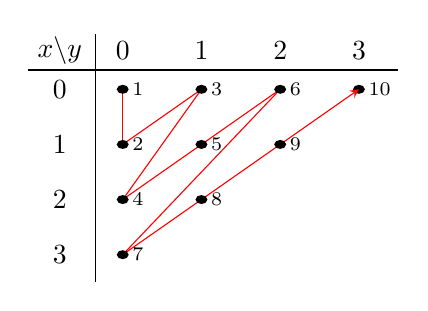
\begin{tikzpicture}[yscale=.7]
			\usetikzlibrary{arrows.meta}
			
			\tikzset{
				myarrow/.style=-stealth
			}
			
			\foreach \x in {0,1,2,3} {
				\node at (.2,-\x-1) {\x};
			}
			\foreach \y in {0,1,2,3} {
				\node at (\y+1,-.3) {\y};
			}
			\draw[red] (1,-1) -- (1,-2);
			\draw[red] (1,-2) -- (2,-1);
			\draw[red] (2,-1) -- (1,-3);
			\draw[red] (1,-3) -- (3,-1);
			\draw[red] (3,-1) -- (1,-4);
			\draw[red] (1,-4) -- (3+.2,-2+.2);
			
			\node at (.2,-.3) {$x\backslash y$};
			\foreach \x in {0,1,2,3} {
				\foreach \y in {0,1,2,3} {
					\ifthenelse{\x<\y \OR \x=\y}{
						\draw[thick,fill] (4-\y,-\x-1) circle (.06);
					}{}
				}
			}
			\draw[myarrow,red] (3+.2,-2+.2) -- (4,-1);
			\node[right] at (1,-1) {\scriptsize 1};
			\node[right] at (1,-2) {\scriptsize 2};
			\node[right] at (2,-1) {\scriptsize 3};
			\node[right] at (1,-3) {\scriptsize 4};
			\node[right] at (2,-2) {\scriptsize 5};
			\node[right] at (3,-1) {\scriptsize 6};
			\node[right] at (1,-4) {\scriptsize 7};
			\node[right] at (2,-3) {\scriptsize 8};
			\node[right] at (3,-2) {\scriptsize 9};
			\node[right] at (4,-1) {\scriptsize 10};
			
			\draw (-.2,-.65) -- (4.5,-.65);
			\draw (.65,0) -- (.65,-4.5);
			
\end{tikzpicture}

	\end{minipage}
\end{center}

Il valore $\langle x,y \rangle$ rappresenta l'incrocio tra la $x$-esima riga e la $y$-esima colonna. Per costruirla:
\begin{enumerate}
	\item $x = 0$
	\item si parte dalla cella $(x,0)$ e si enumerano le celle della diagonale identificata da $(x,0)$ e $(0,x)$
	\item si incrementa $x$ di $1$ e si ripete dal punto precedente
\end{enumerate}

La funzione deve essere: 
\begin{itemize}
	\item iniettiva: non ci possono essere celle con lo stesso numero
	\item suriettiva: ogni numero in $\mathbb{N}^+$ deve comparire
\end{itemize}
Entrambe le proprietà sono soddisfatte, in quanto la numerazione avviene in maniera incrementale, quindi ogni numero prima o poi compare in una cella e di conseguenza ho una coppia che lo genera.\\

\subsubsection{Forma analitica} 
Per la definizione di $\langle x,y \rangle$ si può notare che
$$ \langle x,y \rangle = \langle x + y,0 \rangle + y $$

\begin{center}
	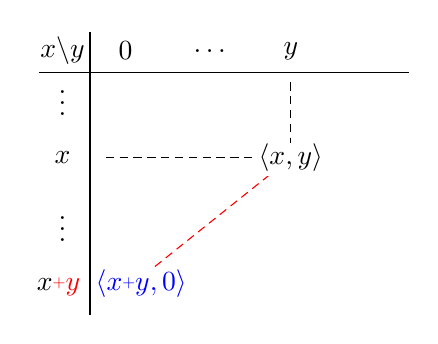
\begin{tikzpicture}[yscale=.8]
		\usetikzlibrary{arrows.meta}
		
		\newcommand{\smallerplus}{\raisebox{.3\height}{\scalebox{.6}{+}}}
		
		\draw[red,densely dashed] (1,-4) -- (3,-2);
		\draw[densely dashed] (.65,-2) -- (3,-2);
		\draw[densely dashed] (3,-1+.2) -- (3,-2);
		
		\node at (.1,-.3) {$x\backslash y$};
		
		\node at (2+1,-.3) {$y$};
		\node at (.9,-.3) {0};
		\node at (1+1,-.3) {$\dots$};
		\node at (.1,-1) {$\vdots$};
		\node at (.1,-1-1) {$x$};
		\node at (.1,-2-1) {$\vdots$};
		\node at (.05,-3-1-.05) {$x{\color{red}\smallerplus y}$};
		\def \offset {.28}
		\draw[white,fill] (3-\offset-.15,-2-\offset) rectangle (3+\offset+.05,-2+\offset-.05);
		\node at (3,-2) {$\langle x,y \rangle$};
		\draw[white,fill] (1-\offset-.15,-4-\offset) rectangle (1+\offset+.05,-4+\offset-.05);
		\node[blue] at (1.1,-4) {$\langle x \smallerplus y, 0 \rangle$};
		
		\draw (-.2,-.65) -- (4.5,-.65);
		\draw (.45,0) -- (.45,-4.5);
\end{tikzpicture}	

\end{center}

Intuitivamente, a partire da $\langle x + y, 0\rangle$ mi basta "salire" seguendo la diagonale fino a $\langle x,y$, ovvero $y$ posti, e per definizione della funzione, $y$ valori più in alto.\\

Il calcolo della funzione coppia si può quindi ridurre al calcolo di $\langle x + y, 0$. Chiamando $x + y = z$, si può notare come ogni cella 
$$ \langle z,0 \rangle = z + \langle z - 1, 0 \rangle $$
E di conseguenza
\begin{align*}
	\langle z,0 \rangle & = z + \langle z - 1, 0 \rangle \\
	& = z + (z-1) + \langle z-2, 0 \rangle \\
	& = z + (z-1) + \dots + 1 + \langle 0,0 \rangle = \\
	& = \sum_{i=1}^{z} i + 1 = \frac{z(z+1)}{2} + 1
\end{align*}

Mettendo insieme le due proprietà viste possiamo ottenere la formula analitica per la funzione coppia: 
$$ \langle x,y \rangle = \langle x + y, 0 \rangle + y = \frac{(x + 1) (x + y + 1)}{2} + y + 1 $$

\subsubsection{Forma analitica di $\sin$ e $\des$} 
Vogliamo fare la stessa cosa per $\sin$ e $\des$, in modo da poter computare l'inversa della funzione coppia, dato $n$. Grazie alle osservazioni precedenti sappiamo che
$$ \begin{array}{r c l}
	\gamma = x + y & \implies & x = \gamma + y \\
	n = y + \langle \gamma , 0 \rangle & \implies & y = n - \langle \gamma , 0 \rangle \\
\end{array} $$

Trovando il valore di $\gamma$ possiamo trovare $x$ e $y$. \\

Notiamo come $\gamma$ sia il più grande valore che, quando calcolato sulla prima colonna ($\langle \gamma, 0 \rangle$) non supera $n$, ovvero
$$ \gamma = \max \{z \in \mathbb{N} | \langle z, 0 \rangle \leq n \} $$
Intuitivamente, si tratta dell'inizio della diagonale che contiene $n$, è "l'inverso" dell'osservazione fatta in precedenza per la quale $ \langle x,y \rangle = \langle x + y,0 \rangle + y $.\\

Risolviamo quindi la disequazione
\begin{align*}
	\langle z, 0 \rangle \leq n & \implies \frac{z(z+1)}{2} + 1 \leq n \\
	& \implies z^2 + z - 2n + 2 \leq 0 \\
	& \implies z_{1,2} = \frac{-1 \pm \sqrt{1 + 8n - 8}}{2} \\
	& \implies \frac{-1 - \sqrt{8n - 7}}{2} \leq z \leq \frac{-1 + \sqrt{8n - 7}}{2} 
\end{align*}

Come valore di $\gamma$ scegliamo
$$ \gamma = \left\lfloor \frac{-1 + \sqrt{8n - 7}}{2} \right\rfloor $$

E con $\gamma$ noto possiamo definire le funzioni $\sin$ e $\des$ come
$$ 
\begin{array}{r c l}
	\des(n) & = & y = n - \langle \gamma, 0 \rangle = n - \frac{\gamma (\gamma + 1)}{2} - 1 \\
	\sin (n) & = & x = \gamma - y
\end{array}
$$

\begin{theor}
	$\mathbb{N} \times \mathbb{N} \sim \mathbb{N}^+$
\end{theor}
\begin{proof}
	La funzione di Cantor è una funzione biettiva tra l'insieme $\mathbb{N} \times \mathbb{N}$ e l'insieme $\mathbb{N}^+$, quindi i due insiemi sono isomorfi.\\
\end{proof}

Possiamo estendere il risultato all'interno dell'insieme $\mathbb{N}$, ovvero:

\begin{theor}
	$\mathbb{N} \times \mathbb{N} \sim \mathbb{N}$
\end{theor}
\begin{proof}
	Definiamo la funzione 
	$$ [,]: \mathbb{N} \times \mathbb{N} \rightarrow \mathbb{N} $$
	tale che
	$$ [x,y] = \langle x,y \rangle - 1$$
	Questa funzione è anch'essa biettiva, quindi i due insiemi sono isomorfi.\\
\end{proof}

Grazie a questo è possibile dimostrare anche che $\mathbb{Q} \sim \mathbb{N}$, infatti i numeri razionali si possono rappresentare come coppie (num, den) e, in generale, tutte le tuple sono isomorfe e $\mathbb{N}$, basta iterare in qualche modo la funzione coppia di Cantor.\\

\subsection{Applicazione alle strutture dati}

I risultati ottenuti fin'ora rendono intuibile come ogni dato possa essere trasformato in un numero, soggetto a trasformazioni matematiche. La dimostrazione \textit{formale} non verrà fatta, anche se verranno fatti esempi di alcune strutture dati che possono essere trasformate in un numero tramite la funzione coppia di Cantor. Ogni struttura dati può essere manipolata e trasformata in una coppia $(x,y)$.\\

Le \textbf{liste} sono le strutture dati più utilizzate nei programmi. In generale non ne è nota la grandezza, di conseguenza è necessario trovare un modo, soprattutto durante l'applicazione di $\sin$ e $\des$, per capire quando abbiamo esaurito gli elementi della lista.\\

Estendiamo la funzione coppia a una lista di interi $x_1, \dots, x_n$:
$$ \langle x_1, \dots, x_n \rangle \rightarrow \langle x_1, \langle x_2 \langle \dots \langle x_n, 0 \rangle \dots \rangle \rangle \rangle $$

Lo $0$ rappresenta il fine lista e non è necessario nel caso in cui il numero di elementi è noto.\\

La decodifica è il processo inverso, partendo dal numero finale si applicano le funzioni $\sin$ e $\des$ ottenendo a ogni iterazione: 
\begin{itemize}
	\item da $\des$ la somma parziale, su cui riapplicare la funzione per ottenere il valore successivo
	\item da $\sin$ il valore presente all'interno della lista
\end{itemize} 
Termina quando il risultato di $\des$ è zero, ovvero l'elemento di fine lista che abbiamo inserito ($x_n$ nel caso di array).
\begin{center}
	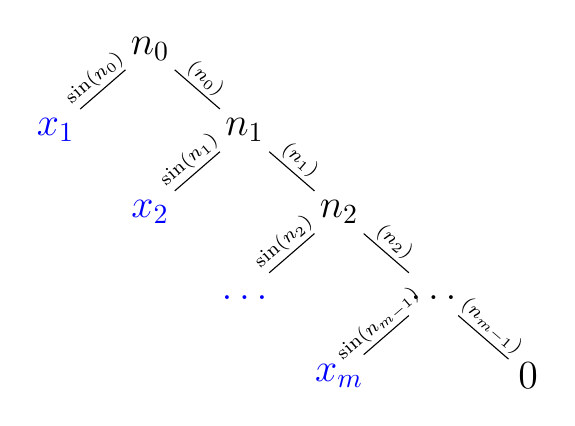
\begin{tikzpicture}[
		level distance=13mm,
		sibling distance=30mm,
		scale=0.8
		]
		\node {\Large$n_0$} 
		child {node[blue] {\Large$x_1$} 
			edge from parent node[xshift=-3,yshift=4,rotate=40.8] {\scriptsize$\sin(n_0)$}
		}
		child {node {\Large$n_1$}
			child {node[blue] {\Large$x_2$}
				edge from parent node[xshift=-3,yshift=4,rotate=40.8] {\scriptsize$\sin(n_1)$}  
			}
			child {node {\Large$n_2$}
				child {node[blue] {\Large$\phantom{n_1}\dots\phantom{n_1}$}
					edge from parent node[xshift=-3,yshift=4,rotate=40.8] {\scriptsize$\sin(n_2)$}  
				}
				child {node {\Large$\phantom{n_1}\dots\phantom{n_1}$}
					child {node[blue] {\Large$x_m$}
						edge from parent node[xshift=-3,yshift=4,rotate=40.8] {\scriptsize$\sin(n_{m-1})$}  
					}
					child {node {\Large$0$} edge from parent 
						node[xshift=3,yshift=4,rotate=-40.8] {\scriptsize$\des(n_{m-1})$}}
					edge from parent node[xshift=3,yshift=4,rotate=-40.8] {\scriptsize$\des(n_2)$}
				}
				edge from parent node[xshift=3,yshift=4,rotate=-40.8] {\scriptsize$\des(n_1)$}
			}
			edge from parent node[xshift=3,yshift=4,rotate=-40.8] {\scriptsize$\des(n_0)$}
		};
\end{tikzpicture}

\end{center}
Se è presente uno 0 all'interno della lista non è un problema in quanto solo $\des$ viene controllato e lo 0 come valore sarà risultato di $\sin$.\\

Quindi è possibile codificare liste e, di conseguenza, \textbf{qualsiasi tipo di dato}, basta convertirlo in una lista di numeri. Per esempio:
\begin{itemize}
	\item una matrice può essere vista come array di array
	\item un grafo può essere rappresentato tramite la sua matrice di adiacenza
	\item i testi sono liste di caratteri
	\item i suoni si possono campionare per ottenere una lista di valori
	\item le immagini sono una "lista" di pixel, ognuno dei quali ha un colore come valore
\end{itemize}

Abbiamo visto come i dati possano essere sostituiti da delle codifiche numeriche; di conseguenza possiamo sostituire tutte le funzioni 
$$ f: \dati \rightarrow \dati \;\; \text{ con funzioni } \;\; f': \mathbb{N} \rightarrow \mathbb{N}_\bot $$

In altre parole, l'universo dei problemi per i quali cerchiamo una soluzione automatica è rappresentabile da $\mathbb{N}_\bot^{\mathbb{N}}$ e di conseguenza $\dati \sim \mathbb{N}$.\\

\section{$\prog \sim \mathbb{N}$}
Adesso lavoriamo sulla parte della relazione che afferma 
$$ F(\C) \sim \prog \sim \mathbb{N} $$

Ovvero, la potenza computazionale (l'insieme dei programmi che un sistema di calcolo $\C$ riesce a calcolare, $F(\C)$) è isomorfa all'insieme di tutti i programmi, a loro volta isomorfi a $\mathbb{N}$.\\

Vogliamo arrivare a ricavare un numero dato un programmo e viceversa. Per farlo servirà vedere l'insieme $\prog$ come l'insieme dei programmi scritti in un certo linguaggio di programmazione.\\

I sistemi analizzati saranno: 
\begin{itemize}
	\item sistema di calcolo $\ram$
	\item sistema di calcolo $\while$
\end{itemize}

Il sistema RAM può apparentemente sembrare "troppo semplice", quindi il sistema WHILE verrà usato per avere un confronto tra le potenze computazionali. Un sistema più sofisticato porta a poter risolvere più problemi? \\

Ci sono due possibili soluzioni: 
\begin{itemize}
	\item $F(\ram \neq F(\while)$: la computabilità \textit{dipende dal sistema usato}
	\item $F(\ram) = F(\while)$: la computabilità è \textit{intrinseca nei problemi} e, di conseguenza, tutti i sistemi sono equivalenti (Tesi di Church-Turing)
\end{itemize}

Il secondo caso è più promettente e, in quel caso, l'obiettivo diventerebbe trovare una \textit{caratterizzazione teorica}, ovvero un "confine" per i problemi calcolabili.\\

\subsection{Sistema di calcolo $\ram$}
Il sistema di calcolo $\ram$ è un sistema semplice che permette di definire rigorosamente: 
\begin{itemize}
	\item $\prog \sim \mathbb{N}$
	\item la \textbf{semantica} dei programmi eseguibili, ovvero $\C(P,\_)$, con $\C = \ram$, ottenendo $\ram (P,\_)$
	\item la \textbf{potenza computazionale}, ovvero calcolare $F(\C)$ con $\C = \ram$, ottenendo $F(\ram)$
\end{itemize}

\subsubsection{Struttura}
Una macchina $\ram$ è formata da un processore e da una memoria teoricamente infinita, divisa in \textbf{celle/registri} contenenti numeri naturali (dati aritmetizzati).\\

Indichiamo i \textbf{registri} con $R_k$, con $k \geq 0$. Tra questi 
\begin{itemize}
	\item $R_0$ contiene l'output
	\item $R_1$ contiene l'input
\end{itemize}

Inoltre è presente un registro $L$, anche detto \textbf{program counter} $PC$ che indica l'indirizzo dell'istruzione successiva.\\

Dato un \textbf{programma} $P$, indichiamo con $|P|$ il numero di istruzioni che il programma contiene.\\

Le \textbf{istruzioni} nel linguaggio RAM sono: 
\begin{itemize}
	\item \textbf{incremento}: $R_k \leftarrow R_k + 1$
	\item \textbf{decremento}: $R_k \leftarrow R_k - 1$
	\item \textbf{salto condizionato}: \texttt{if $R_k = 0$ then goto $m$}, con $m \in \{1, \dots, |P|\}$
\end{itemize}
L'istruzione di decremento è tale che
$$ x - y = \begin{cases}
	x-y & \text{ se } x \geq y\\
	0 & \text{ altrimenti }
\end{cases}$$

\begin{center}
	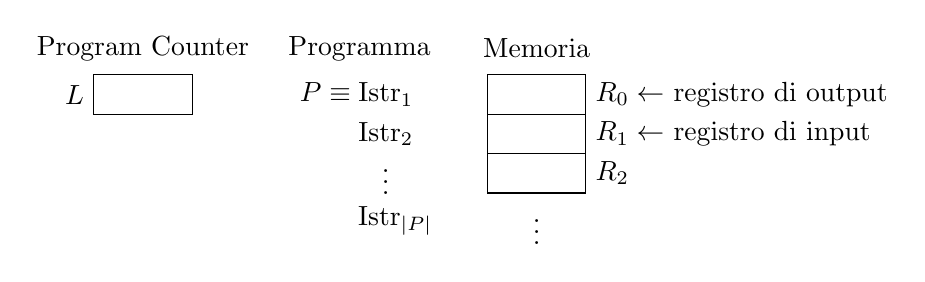
\begin{tikzpicture}
    \node[above] at (.875,.6) {Memoria};

    \draw (.25,0) rectangle (1.5,.5);
    \node[right] at (1.5,.25) {$R_0 \leftarrow$ registro di output};
    \draw (.25,-.5) rectangle (1.5,0);
    \node[right] at (1.5,-.25) {$R_1 \leftarrow$ registro di input};
    \draw (.25,-1) rectangle (1.5,-.5);
    \node[right] at (1.5,-.75) {$R_2$};
    
    \node[below] at (.875,-1) {$\vdots$};

    \def\y{2.25}
    \node[above] at (.875-\y,.55) {Programma};
    \node[] at (.84-\y,.25) {$P\equiv\text{Istr}_1$};
    \node[] at (1.21-\y,-.25) {$\text{Istr}_2$};
    \node[] at (1.21-\y,-.75) {$\vdots$};
    \node[] at (1.33-\y,-1.35) {$\text{Istr}_{|P|}$};

    \def\x{5}
    \node[above] at (.875-\x,.55) {Program Counter};

    \draw (.25-\x,0) rectangle (1.5-\x,.5);
    \node[left] at (1.5-1.25-\x,.25) {$L$};
\end{tikzpicture}

\end{center}

\subsubsection{Esecuzione di un programma RAM}

L'esecuzione di un programma su una macchina RAM segue i passi:
\begin{enumerate}
	\item \textbf{Inizializzazione}:
	\begin{itemize}
		\item viene caricato il programma $P \equiv \text{Istr}_1, \dots \text{Istr}_n$ in memoria
		\item il PC viene posto a 1 per indicare di eseguire la prima istruzione del programma
		\item viene caricato l'input in $R_1$
		\item ogni altro registro è azzerato
	\end{itemize}
	\item \textbf{Esecuzione}: le istruzioni vengono eseguite una dopo l'altra, a ogni iterazione passa da $L$ a $L+1$ (escluse operazioni di salto). Essendo il linguaggio RAM \textit{non strutturato} richiede un PC per sapere l'operazione da eseguire al passo successivo.
	\item \textbf{Terminazione}: per convenzione, si usa $L=0$ per indicare che l'esecuzione del programma è terminata o andata in loop. Nel caso in cui il programma termini, è detto \textbf{segnale di halt} e arresta la macchina
	\item \textbf{Output}: il contenuto di $R_0$, in caso di halt, contiene il risultato dell'esecuzione del programma $P$. Si indica con $\varphi_P(n)$ il contenuto del registro $R_0$ in caso di halt, oppure $\bot$ in caso di loop
	$$ 
	\varphi_P (n) = \begin{cases}
		cont(R_0) & \text{ se halt} \\
		\bot & \text{ se loop}
	\end{cases}
	$$
\end{enumerate}
Con $\varphi_P: \mathbb{N} \rightarrow \mathbb{N}_\bot$ indichiamo la semantica del programma $P$.\\

Con $\C(P,\_)$ indicavamo la semantica di $P$ nel sistema di calcolo $\C$, quindi con $\ram(P,\_) = \varphi_P$ indichiamo la semantica di $P$ nel sistema di calcolo RAM.\\

\subsubsection{Semantica Operazionale}

Per dare una definizione formale della semantica di un programma RAM va specificato il significato di ogni istruzione (\textbf{semantica operazionale}), esplicitando l'effetto che quell'istruzione ha sui registri della macchina.\\

Ogni istruzione fa passare la macchina da uno stato all'altro e la \textbf{semantica operazionale} di un'istruzione è la \textbf{coppia} formata dagli \textbf{stati} della macchina \textbf{prima e dopo l'istruzione}.
$$ \text{STATO}_1 \rightarrow \boxed{\text{Istr}_i} \rightarrow \text{STATO}_2 $$
$$ (\text{STATO}_1,\text{STATO}_2) = \text{semantica operazionale di Istr}_i $$

Uno stato deve descrivere completamente la situazione della macchina in un certo istante. Il programma rimane uguale, quindi l'informazione da salvare è la situazione globale dei registri $R_k$ e il registro $L$.\\

La \textbf{computazione} del programma $P$ è una sequenza di stati $\st_i$, ognuno generato dall'esecuzione di un'istruzione del programma; $P$ induce una sequenza di stati $\st_i$, se questa è formata da un numero infinito di stati, allora il programma è andato in loop; in caso contrario, nel registro $R_0$ si trova il risultato $y$ della computazione di $P$.
$$ 
\varphi_P: \mathbb{N} \rightarrow \mathbb{N}_\bot \tc \varphi_P(n) = \begin{cases}
	y & \text{ se } \exists \st_{fin} \\
	\bot & \text{ altrimenti}
\end{cases}
$$

Per definire come passare da uno stato all'altro, definiamo formalmente: 
\begin{itemize}
	\item \textbf{Stato}: istantanea di tutte le componenti della macchina, è una funzione 
	$$ \st: \{L, R_i\} \rightarrow \mathbb{N} $$
	tale che $\st (R_k)$ restituisce il contenuto del registro $R_k$ quando la macchina si trova nello stato $\st$. Gli stati possibili di una macchina appartengono all'insieme 
	$$ \stati = \{f: \{L, R_i\} \rightarrow \mathbb{N}\} = \mathbb{N}^{\{L,R_i\}} $$
	%Questa rappresentazione permette un numero di registri potenzialmente infinito. Se così non fosse, avremmo tuple per indicare tutti i possibili registri al posto dell'insieme $\{L,R_i\}$
	
	\item \textbf{Stato Finale}: uno stato finale $\st_{fin}$ è un qualsiasi stato $\st$ tale che $\st (L) = 0$
	\item \textbf{Dati}: già dimostrato come $\dati \sim \mathbb{N}$
	\item \textbf{Inizializzazione}: serve una funzione che, preso l'input, restituisca lo stato iniziale della macchina: 
	$$ \text{in}: \mathbb{N} \rightarrow \stati \tc \text{in}(n) = \st_{init}$$
	Lo stato iniziale $\st_{init}$ è tale che 
	$$ 
	\st_{init} (R) = \begin{cases}
		1 & \text{ se } R=L \\
		n & \text{ se } R=R_1 \\
		0 & \text{ altrimenti}
	\end{cases}
	$$
	\item \textbf{Programmi}: $\prog$ è definito come l'insieme dei programmi $\ram$
\end{itemize}

Manca da definire la \textit{parte dinamica} del programma, ovvero l'esecuzione. Per farlo, definiamo la \textbf{funzione di stato prossimo}: 
$$ \delta : \stati \times \prog \rightarrow \stati_\bot $$
tale che 
$$ \delta (\st,P) = \st' $$
dove $\st$ rappresenta lo stato attuale e $\st'$ rappresenta lo stato prossimo dopo l'esecuzione di un'istruzione di $P$.\\

La funzione $\delta (\st, P) = \st'$ è tale che
\begin{itemize}
	\item se $\st(L) = 0$ ho halt, ovvero deve terminare la computazione. Poniamo lo stato come indefinito, ovvero $\st' = \bot$
	\item Se $\st(L)>|P|$ vuol dire che $P$ non contiene istruzioni che bloccano esplicitamente l'esecuzione del programma. Lo stato $\st'$ è tale che 
	$$ 
	\st'(R) = \begin{cases}
		0 & \text{ se } R = L \\
		\st(R_i) \text{ se } R = R_i \forall i
	\end{cases}
	$$
	\item Se $1 \leq \st(L) \leq |P|$ considero l'istruzione $\st(L)$-esima:
	\begin{itemize}
		\item se ho un incremento/decremento sul registro $R_k$ definisco $\st'$ tale che 
		$$ 
		\begin{cases}
			\st'(L) & = \st (L) + 1\\
			\st'(R_k) & = \st (R_k) \pm 1\\
			\st'(R_i) & = \st (R_i) \; \text{ per } \; i \neq k \\
		\end{cases}
		$$
		\item Se ho un \texttt{goto} sul registro $R_k$ che salta all'indirizzo $m$, definisco $\st'$ tale che 
		$$ 
		\st' (L) = \begin{cases}
			m & \text{ se } \st (R_k) = 0 \\
			\st (L) + 1 & \text{ altrimenti}
		\end{cases}
		$$
		$$ \st' (R_i) = \st (R_i) \; \forall i $$
	\end{itemize}
\end{itemize}

L'esecuzione di un programma $P \in \prog$ su input $n \in \mathbb{N}$ genera una sequenza di stati 
$$ \st_0, \st_1, \dots, \st_i, \st_{i+1}, \dots $$
tali che 
$$
\begin{array}{l l c l}
	& \st_0 & = & \text{in}(n) \\
	\forall i & \st_{i+1} & = & \delta (\st_i,P) 
\end{array}
$$
La sequenza è infinita quando $P$ va in loop, mentre se termina raggiunge uno stato $\st_m$ tale che $\st_m (L) = 0$, ovvero ha ricevuto il segnale di halt. \\

La semantica di $P$ è 
$$ 
\varphi_P (n) = \begin{cases}
	y & \text{ se } P \text{ termina in } \st_m, \text{ con } \st_m (L) = 0 \text{ e } \st_m(R_0) = y \\
	\bot & \text{ se } $P$ \text{ va in loop}
\end{cases}
$$

La potenza computazionale del sistema $\ram$ è 
$$ F(\ram) = \left\{f \in \mathbb{N}^{\mathbb{N}}_\bot | \exists P \in \prog | \varphi_P = f \right\} = \left\{\varphi_P | P \in \prog \right\} \subsetneq \mathbb{N}^{\mathbb{N}}_\bot $$
L'insieme è formato da tutte le funzioni $f: \mathbb{N} \rightarrow \mathbb{N}_\bot$ che hanno un programma che le calcola in un sistema $\ram$.\\

\subsection{Aritmetizzazione di un programma}

Per verificare che $\prog \sim \mathbb{N}$ basterebbe trovare una funzione che permetta di codificare i programmi in numeri in modo biunivoco. Data una lista di istruzioni semplici $P \equiv \text{Istr}_1, \dots, \text{Istr}_m$ se questa fosse codificata come una lista di interi potremmo sfruttare la funzione coppia di Cantor per ottenere un numero associato al programma $P$.\\

Quindi vogliamo trovare una funzione $Ar$ che associ a ogni istruzione $I_k$ la sua codifica numerica $c_k$. Se la funzione trovata è anche biunivoca siamo sicuri di poter trovare anche la sua inversa, ovvero la funzione che ci permette di ricavare $I_k$ da $c_k$.\\

Riassumendo, vogliamo trasformare la lista di istruzioni un una lista di numeri su cui successivamente applicare la funzione coppia di Cantor. Vorremmo anche ottenere la lista di istruzioni originale data la codifica.
\begin{center}
	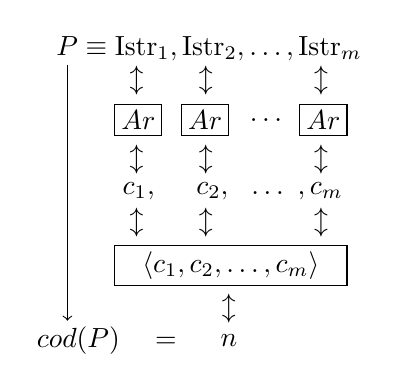
\begin{tikzpicture}
    \node at (0,0)
        {$ P \equiv \text{Istr}_1,\text{Istr}_2,\dots,\text{Istr}_m$};
    \node at (.25,-.4) 
        {$\updownarrow \qquad \updownarrow \qquad \ \ \ \ \ \updownarrow$};
    
    \draw (-1.2,-1.1) rectangle (-.6,-.7) node[midway] {$Ar$};
    \begin{scope}[xshift=.85cm]
        \draw (-1.2,-1.1) rectangle (-.6,-.7) node[midway] {$Ar$};
    \end{scope}
    \begin{scope}[xshift=2.35cm]
        \draw (-1.2,-1.1) rectangle (-.6,-.7) node[midway] {$Ar$};
    \end{scope}
    \node at (.75,-.9) {$\dots$};

    \node at (.25,-1.4) 
        {$\updownarrow \qquad \updownarrow \qquad \ \ \ \ \ \updownarrow$};
    \node at (.3,-1.8) 
        {$c_1,\ \ \ \ c_2, \ \ \dots \  ,c_m$};
    \node at (.25,-2.2) 
        {$\updownarrow \qquad \updownarrow \qquad \ \ \ \ \ \updownarrow$};
    \draw (-1.2,-3) rectangle (1.75,-2.5) node[midway] 
        {$\langle c_1,c_2,\dots,c_m \rangle$};
    \node at (.25,-3.3) {$\updownarrow$};
    \node at (.25,-3.7) {$n$};
    \node at (-1.3,-3.7) {$cod(P) \quad =$};
    \draw [->] (-1.8,-.2) -- (-1.8,-3.45);

\end{tikzpicture}

\end{center} 
L'associazione biunivoca di un numero a una struttura si dice aritmetizzazione o G\"odelizzazione.\\

\subsubsection{Applicazione ai programmi RAM}
Dovendo codificare tre istruzioni nel linguaggio $\ram$, definiamo la funzione $Ar$ tale che
$$ 
Ar(I) = \begin{cases}
	3k & \text{ se } I \equiv R_k \leftarrow R_k + 1 \\
	3k + 1 & \text{ se } I \equiv R_k \leftarrow R_k \dotminus 1 \\
	3k \langle k,m\rangle - 1 & \text{ se } I \equiv \text{ \texttt{if} } R_k = 0 \text{ \texttt{then goto} } m \\
\end{cases}
$$
Per l'inversa, in base al modulo tra $n$ e 3 ottengo una certa istruzione: 
$$
Ar^{-1} (n) = \begin{cases}
	R_{\frac{n}{3}} \leftarrow R_{\frac{n}{3}} + 1 & \text{ se } n \mod 3 = 0 \\
	R_{\frac{n-1}{3}} \leftarrow R_{\frac{n-1}{3}} \dotminus 1 & \text{ se } n \mod 3 = 1 \\
	\text{\texttt{if} } R_{\sin\left(\frac{n+1}{3}\right)} = 0 \text{ \texttt{then goto} } \des\left(\frac{n+1}{3}\right) & \text{ se } n \mod 3 = 2 \\
\end{cases}
$$

Per tornare indietro devo prima invertire la funzione coppia di Cantor e poi invertire la funzione $Ar$.\\
La lunghezza del programma $P$, indicata con $|P|$, si calcola come $len(cod(P))$.\\

Abbiamo quindi dimostrato che $\prog \sim \mathbb{N}$.\\

\subsubsection{Osservazioni}
Avendo $n = cod(P)$ si può scrivere
$$ \varphi_P (t) = \varphi_n (t) $$
Ovvero, la semantica di $P$ è uguale alla semantica della sua codifica. \\

I numeri diventano un \textit{linguaggio di programmazione}.\\

Si può scrivere l'insieme 
$$ F(\ram) = \{\varphi_P: P \in \prog \}$$
come 
$$ F(\ram) = \{\varphi_i\}_{i \in \mathbb{N}} $$
L'insieme, grazie alla dimostrazione di $\prog \sim \mathbb{N}$, è numerabile.\\

Abbiamo dimostrato rigorosamente che 
$$ F(\ram) \sim \mathbb{N} \nsim \mathbb{N}^{\mathbb{N}}_\bot $$
Di conseguenza, anche nel sistema di calcolo $\ram$ esistono funzioni no calcolabili.\\

La $\ram$ è troppo elementare affinché $F(\ram)$ rappresenti formalmente la "classe dei problemi risolubili automaticamente", quindi considerando un sistema di calcolo $\C$ più sofisticato, ma comunque trattabile rigorosamente come il sistema $\ram$, potremmo dare un'idea formale di "ciò che è calcolabile automaticamente".\\

Se riesco a dimostrare che $F(\ram) = F(\C)$ allora cambiare la tecnologia non cambia ciò che è calcolabile, ovvero la calcolabilità è intrinseca ai problemi, quindi la si può caratterizzare matematicamente. \\

\subsection{Sistema di calcolo $\while$}
Introduciamo quindi il sistema di calcolo $\while$ per vedere se riusciamo a "catturare" più o meno funzioni calcolabili dalla macchina $\ram$.

\subsubsection{Struttura}
La macchina $\while$ ha anch'essa, come la macchina $\ram$, una serie di registri, ma al posto di essere \textit{potenzialmente infiniti} sono esattamente 21. Il registro $R_0$ è il \textbf{registro di output}, mentre $R_1$ è il \textbf{registro di input}. Non esiste il Program Counter in quanto il linguaggio è \textbf{strutturato} e ogni istruzione in questo linguaggio va eseguita in ordine.\\

Il linguaggio $\while$ prevede una \textbf{definizione induttiva}: vengono definiti alcuni comandi base e i comandi più complessi sono una concatenazione dei comandi base.\\

\paragraph{Assegnamento:} Comando di base, ne esistono di tre tipi: 
\begin{align*}
	x_k & := 0, \\
	x_k & := x_j + 1 \\
	x_k & := x_j \dotminus 1
\end{align*}
Queste istruzioni sono più complete rispetto alle istruzioni $\ram$, in una sola istruzione possiamo azzerare il valore di una variabile o assegnare a una variabile il valore di un'altra aumentato/diminuito di 1.

\paragraph{While:} Primo comando "induttivo". Si tratta di un comando della forma: 
\begin{center}
	\texttt{while} $x_k \neq 0$ \texttt{do} $C$
\end{center}
Dove $C$ è detto \textbf{corpo} e può essere un assegnamento, un comando while o un comando composto.

\paragraph{Composto:} Altro comando induttivo. Si tratta di un comando nella forma
\begin{center}
	\texttt{begin} $C_1; \dots; C_n$ \texttt{end}
\end{center}
Dove i vari $C_i$ sono, come prima, assegnamenti, comandi while o comandi composti.\\

\paragraph{Programma $\while$:} Un programma $\while$ è un comando composto, e l'insieme di tutti i programmi $\while$ è l'insieme
$$ W-\prog = \{\prog \text{ scritti in linguaggio } \while \} $$

Chiamiamo 
$$ \Psi_W : \mathbb{N} \rightarrow \mathbb{N}_\bot $$
la \textbf{semantica} del programma $W \in W-\prog$.\\

Per dimostrare una proprietà $P$ di un programma $W \in W-\prog$, data la definizione induttiva del linguaggio $\while$, è naturale procedere induttivamente: 
\begin{enumerate}
	\item dimostro $P$ vera sugli assegnamenti 
	\item suppongo $P$ vera sul comando $C$ e la dimostro vera per \texttt{while $x_k \neq 0$ do $C$}
	\item suppongo $P$ vera sui comandi $C_1, \dots, C_n$ e la dimostro vera per \texttt{begin $C_1; \dots; C_n$ end}
\end{enumerate}

\subsubsection{Esecuzione di un programma $\while$}
L'esecuzione di un programma $\while$ $W$ è composta dalle seguenti fasi: 
\begin{enumerate}
	\item \textbf{Inizializzazione}: ogni registro $x_i$ viene posto a $0$, tranne $x_1$, che contiene l'input $n$
	\item \textbf{Esecuzione}: essendo $\while$ un linguaggio con strutture di controllo, non serve un Program Counter, poiché le istruzioni di $W$ vengono eseguite l'una dopo l'altra
	\item \textbf{Terminazione}: l'esecuzione di $W$ può 
	\begin{itemize}
		\item \textit{arrestarsi}: se arriva al termine delle istruzioni
		\item \textit{non arrestarsi}: se entra in un loop
	\end{itemize}
	\item \textbf{Output}: Se il programma va in halt, l'output è contenuto nel registro $x_0$. Possiamo scrivere
	$$ \Psi_W (n) = \begin{cases}
		cont(x_0) & \text{ se halt} \\
		\bot & \text{ se loop}
	\end{cases}$$
\end{enumerate}

\subsubsection{Definizione formale per l'esecuzione}
Come per i programmi $\ram$, serve una definizione formale per la semantica di un programma $\while$, per la quale servono una serie di elementi
\begin{itemize}
	\item \textbf{Stato}: una tupla grande quanto il numero di variabili, dove quindi $\underline{x} = (c_0, \dots, c_{20})$ rappresenta uno stato, con $c_i$ rappresentante il contenuto della variabile $i$
	\item \textbf{$\wstati$}: Insieme di tutti gli stati possibili, contenuto in $\mathbb{N}^{21}$ vista la definizione degli stati 
	\item \textbf{Dati}: già visto che $\dati \sim \mathbb{N}$
	\item \textbf{Inizializzazione}: Lo stato iniziale è descritto dalla funzione 
	$$ w\text{-}in(n) = (0, n, 0, \dots, 0) $$
	\item \textbf{Semantica operazionale}: Vogliamo trovare una funzione che, presi comando da eseguire e stato corrente, restituisce lo stato successivo
\end{itemize}

\paragraph{Funzione stato prossimo:} Soffermandoci sull'ultimo punto, vogliamo trovare la funzione
$$  \llbracket \rrbracket (): \wcom \times \wstati \rightarrow \wstati_\bot $$
Che, dati un comando $C$ del linguaggio $\while$ e lo stato corrente $\underline{x}$, calcoli
$$ \llbracket C \rrbracket (\underline{x}) = \underline{y} $$
con $\underline{y}$ stato prossimo. Quest'ultimo dipende dal comando $C$, ma essendo $C$ induttivo, possiamo provare a dare una definizione induttiva della funzione.\\

Partendo dal passo base, gli \textbf{assegnamenti}:
$$
\llbracket x_k := 0 \rrbracket (\underline{x}) = \underline{y} = \begin{cases}
	x_i & \text{ se } i \neq k \\
	0 & \text{ se } i = k
\end{cases}
$$
$$ 
\llbracket x_k := x_j \pm 1 \rrbracket (\underline{x}) = \underline{y} = \begin{cases}
	x_i & \text{ se } i \neq k \\
	x_j \pm 1 & \text{ se } i = k
\end{cases}
$$

Proseguiamo con il \textbf{passo induttivo}:
\begin{itemize}
	\item \textbf{Comando composto}: vogliamo calcolare
	$$ \llbracket \text{\texttt{begin }} C_1; \dots; C_n \text{\texttt{ end}} \rrbracket (\underline{x}) $$
	Conoscendo ogni $\llbracket C_i \rrbracket$ per ipotesi induttiva, calcoliamo la funzione
	$$ \llbracket C_n \rrbracket \left(\dots \left(\llbracket C_2 \rrbracket \left(\llbracket C_1 \rrbracket (\underline{x})\right)\right) \dots \right) = \left(\llbracket C_n \rrbracket \circ \dots \circ \llbracket C_1 \rrbracket \right) (\underline{x}) $$
	Ovvero, applichiamo in ordine i comandi $C_i$ presenti nel comando composto $C$
	
	\item \textbf{Comando while}: vogliamo calcolare
	$$ \llbracket \text{\texttt{while }} x_k \neq 0 \text{ \texttt{do} } C \rrbracket (\underline{x}) $$
	Conoscendo ogni $\llbracket C_i \rrbracket$ per ipotesi induttiva, calcoliamo la funzione 
	$$ \llbracket C \rrbracket \left(\dots \left(\llbracket C \rrbracket (\underline{x})\right) \dots \right) $$
	Bisogna capire quante volte eseguire il ciclo: dato $\llbracket C \rrbracket^e$ (comando $C$ eseguito $e$ volte) vorremmo trovare il valore di $e$. Questo è il numero minimo di iterazioni che portano in uno stato in cui $x_k = 0$, ovvero il comando \texttt{while} diventa
	$$ \text{\texttt{while} } x_k \neq 0 \text{ \texttt{do} } C = \begin{cases}
		\llbracket C \rrbracket^e (\underline{x}) & \text{ se } e = \mu_t \\
		\bot & \text{ altrimenti}
	\end{cases}$$
	Il valore $e = \mu_t$ è quel numero tale che $\llbracket C \rrbracket^e (\underline{x})$ ha  la $k$-esima componente dello stato uguale a 0
\end{itemize}

Definita la semantica operazionale, manca solo da definire cos'è la \textbf{semantica del programma} $W$ su input $n$. Questa è la funzione 
$$ \Psi_W: \mathbb{N} \rightarrow \mathbb{N}_\bot \; | \; \Psi_W (n) = \text{Proj}\left(0, \llbracket W \rrbracket (w\text{-}in(n))\right)$$

Questo è valido in quanto $W$ programma $\while$ è un programma composto, e abbiamo definito come deve comportarsi la funzione $\llbracket \rrbracket ()$ sui comandi composti.\\

\paragraph{Potenza Computazionale:} La potenza computazionale del sistema di calcolo $\while$ è l'insieme 
$$ F(\while) = \left\{f \in \mathbb{N}^{\mathbb{N}}_\bot | \exists W \in \wprog | f = \Psi_W \right\} = \left\{\Psi_W : W \in \wprog \right\}$$

Ovvero, l'insieme formato da tutte le funzioni che possono essere calcolate con un programma in $\wprog$.\\

\subsection{Confronto tra macchina $\ram$ e $\while$}
Viene naturale confrontare i due sistemi presentati per capire il "più potente", sempre che ce ne sia uno. Le possibilità sono: 
\begin{itemize}
	\item $F(\ram) \subsetneq F(\while)$, data l'estrema semplicità del sistema $\ram$
	\item $F(\ram) \cap F(\while) = \emptyset$, avere insiemi disgiunti significherebbe che il concetto di calcolabile dipende dalla macchina considerata
	\item $F(\while) \subseteq F(\ram)$, che sarebbe sorprendente vista l'apparente maggiore sofisticatezza del sistema $\while$
	\item $F(\while) = F(\ram)$, ovvero il concetto di calcolabile non dipende dalla tecnologia utilizzata ma è intrinseco nei problemi
\end{itemize}

\paragraph{Confronto tra sistemi di calcolo:} Ponendo di avere $\C_1$ e $\C_2$ sistemi di calcolo con programmi in $\cprog{1}$ e $\cprog{2}$ e le relative potenze computazionali
$$ F(\C_1) = \left\{f: \mathbb{N} \rightarrow \mathbb{N}_\bot | \exists P_1 \in \cprog{1} | f = \Psi_{P_1} \right\} = \left\{\Psi_{P_1}: P_1 \in \cprog{1} \right\} $$
$$ F(\C_2) = \left\{f: \mathbb{N} \rightarrow \mathbb{N}_\bot | \exists P_2 \in \cprog{2} | f = \Psi_{P_2} \right\} = \left\{\Psi_{P_2}: P_2 \in \cprog{2} \right\} $$

Mostrare che il primo sistema non è più potente del secondo $F(\C_1) \subseteq F(\C_2)$ vuol dire dimostrare che ogni elemento nel primo insieme deve stare anche nel secondo
$$ \forall f \in F(\C_1) \implies f \in F(C_2) $$

\textit{Espandendo} la definizione di $f \in F(\C)$ la relazione diventa
$$ \forall P_1 \in \cprog{1} | f = \Psi_{P_1} \implies \exists P_2 \in \cprog{2} | f = \Psi_{P_2} $$

Per ogni programma calcolabile nel primo sistema di calcolo ne esiste uno con la stessa semantica nel secondo sistema. Vogliamo trovare un \textbf{compilatore} (o \textbf{traduttore}), ovvero una funzione che trasformi un programma del primo sistema in uno del secondo.\\

\subsubsection{Traduzioni}
Dati $\C_1$ e $\C_2$ due sistemi di calcolo, definiamo \textbf{traduzione} da $\C_1$ a $\C_2$ una funzione
$$ T: \cprog{1} \rightarrow \cprog{2} $$

Con le seguenti proprietà:
\begin{itemize}
	\item \textbf{programmabile}: esiste un modo per programmarla
	\item \textbf{completa}: deve saper tradurre \textit{ogni} programma in $\cprog{1}$ in un programma in $\cprog{2}$
	\item \textbf{corretta}: mantiene la semantica dei programmi di partenza, ovvero
	$$ \forall P \in \cprog{1} \;\; \Psi_P = \varphi_{T(P)}$$
	dove $\Psi$ rappresenta la semantica dei programmi in $\cprog{1}$ e $\varphi$ rappresenta la semantica dei programmi in $\cprog{2}$\\
\end{itemize}


\begin{theor}
	Se esiste $T: \cprog{1} \rightarrow \cprog{2}$ allora $F(\C_1) \subseteq F(\C_2)$
\end{theor}
\begin{proof}
	Se $f \in F(\C_1)$ allora esiste un programma $P_1 \in \cprog{1}$ tale che $\Psi_{P_1} = f$.\\
	
	A questo programma $P_1$ applico $T$, ottenendo $T(P_1) = P_2 \in \cprog{2}$ (per \textit{completezza}) tale che $\varphi_{P_2} = \Psi_{P_1} = f$ (per \textit{correttezza}).\\
	
	Ho trovato un programma $P_2 \in \cprog{2}$ la cui semantica è $f$, allora $F(\C_1) \subseteq F(\C_2)$.\\
\end{proof}

Mostreremo che $F(\while) \subseteq F(\ram)$, ovvero che il sistema $\while$ non è più potente del sistema $\ram$. Costruiremo un compilatore
$$ \comp: \wprog \rightarrow \prog $$
che rispetti le caratteristiche di programmabilità, completezza e correttezza.\\

\subsection{$F(\while) \subseteq F(\ram)$}

Per provare che $F(\while) \subseteq F(\ram)$ vogliamo costruire un compilatore da $\while$ a $\ram$.\\

Per comodità, introduciamo un linguaggio $\ram$ \textit{etichettato}: aggiunge la possibilità di etichettare un'istruzione che indica un punto di salto o di arrivo (stile label assembly). Non altera la potenza espressiva del linguaggio in quanto si tratta di un'aggiunta puramente sintattica: il $\ram$ etichettato si traduce facilmente in $\ram$ puro.\\

Essendo $\wprog$ un insieme definito induttivamente, possiamo definire induttivamente anche il compilatore:
\begin{itemize}
	\item \textbf{Passo base}: come compilare gli assegnamenti
	\item \textbf{Passo induttivo}:
	\begin{enumerate}
		\item Per I.H., assumo di sapere $\comp(C_1), \dots, \comp(C_m)$ e mostro come compilare il comando composto \texttt{begin $C_1; \dots; C:n$ end}
		\item Per I.H., assumo di sapere $\comp(C)$ e mostro come compilare il comando \texttt{while $x_k \neq 0$ do $C$}
	\end{enumerate}
\end{itemize}

Nelle traduzioni andremo a mappare la variabile $\while$ $x_k$ nel registro $\ram$ $R_k$. Questo non crea problemi in quanto stiamo mappando un numero finito di registri in un insieme infinito.\\

Il primo assegnamento che mappiamo è $x_k := 0$
\begin{center}
	\renewcommand{\arraystretch}{1.25}
	\begin{tabular}{l|r l|}
		\cline{2-3}
		$\comp(x_k:=0) =$ & \texttt{LOOP}:& \texttt{IF $R_k = 0$ THEN GOTO EXIT}\\
		&& $R_k\leftarrow R_k \dotminus 1$ \\
		&& \texttt{IF $R_{21} = 0$ THEN GOTO LOOP} \\
		&\texttt{EXIT}:& $R_k \leftarrow R_k \dotminus 1$ \\
		\cline{2-3}
	\end{tabular}\vspace{.15cm}
\end{center}

Questo programma $\ram$ azzera il valore di $R_k$ usando il registro $R_{21}$ per saltare al check della condizione iniziale. Viene utilizzato il registro $R_{21}$ perché, non essendo mappato a nessuna variabile $\while$, sarà sempre nullo dopo la fase di inizializzazione.\\

Gli altri due assegnamenti da mappare sono $x_k:= x_j+1$ e $x_k := x_j \dotminus 1$:
\begin{itemize}
	\item Se $k=j$, la traduzione è banale e l'istruzione $\ram$ è
	$$ \comp(x_k := x_k \pm 1) = R_k \leftarrow R_k \pm 1 $$
	\item Invece se $k \neq j$ la prima idea è quella di "spostare" $x_j$ in $x_k$ e poi fare $\pm 1$ ma non funziona per due ragioni
	\begin{enumerate}
		\item se $R_k \neq 0$ la migrazione (quindi sommare $R_j$ a $R_k$) non genera $R_j$ dentro $R_k$. Si può risolvere azzerando il registro $R_k$ prima della migrazione
		\item $R_j$ dopo il trasferimento è ridotto a 0, ma questo non è il senso dell'istruzione, vorrei solo "\textit{fotocopiarlo}" dentro $R_k$. Questo può essere risolto salvando $R_j$ in un altro registro, azzerare $R_k$, spostare $R_j$ e ripristinare il valore originale di $R_j$
	\end{enumerate}
%	Ricapitolando: 
%	\begin{itemize}
%		\item salviamo $x_j$ in $R_{22}$, registro \textit{sicuro} perché mai coinvolto in altre istruzioni
%		\item azzeriamo $R_k$
%		\item Rigeneriamo $R_j$ e settiamo $R_k$ da $R_{22}$
%		\item $\pm 1$ in $R_k$
%	\end{itemize}
	Quindi possiamo mappare come:
	\begin{center}
		\renewcommand{\arraystretch}{1.25}
		\begin{tabular}{l|r l|l}\cline{2-3}
			$\comp (x_k := x_j \pm 1)$: & \texttt{LOOP}:& \texttt{IF $R_j = 0$ THEN GOTO E1}
			&\multirow{4}{*}{\hspace{-.2cm}
				$\begin{rcases}
					\phantom{}\\
					\phantom{}\\
					\phantom{}\\
					\phantom{}\\
				\end{rcases}$ Salva $R_j$ in $R_{22}$
			} \\
			&& $R_j\leftarrow R_j \dotminus 1$ & \\
			&& $R_{22} \leftarrow R_{22} + 1$ & \\
			&& \texttt{IF $R_{21} = 0$ THEN GOTO LOOP} & \\
			& \texttt{E1:} & \texttt{IF $R_k = 0$ THEN GOTO E2} &\multirow{3}{*}{\hspace{-.2cm}
				$\begin{rcases}
					\phantom{}\\
					\phantom{}\\
					\phantom{}\\
				\end{rcases}$ Azzera $R_k$
				}\\
			&& $R_k \leftarrow R_k \dotminus 1$ & \\
			&& \texttt{IF $R_{21} = 0$ THEN GOTO EXIT 1} & \\
			& \texttt{E2} & \texttt{IF $R_{22} = 0$ THEN GOTO E3} & \multirow{4}{*}{\hspace{-.2cm} 
			$\begin{rcases}
				\phantom{}\\
				\phantom{}\\
				\phantom{}\\
				\phantom{}\\
				\phantom{}\\
			\end{rcases}$ Rigenera $R_j$ e $R_k$ da $R_{22}$
			} \\
			&& $R_k \leftarrow R_k + 1$ & \\
			&& $R_j \leftarrow R_j + 1$ & \\
			&& $R_{22} \leftarrow R_{22} \dotminus 1$ & \\
			&& \texttt{IF $R_{21} = 0$ THEN GOTO E2} & \\ 
			& \texttt{E3:} & $R_k \leftarrow R_k \pm 1$ & \\
			\cline{2-3} 
		\end{tabular}\vspace{.5cm}
	\end{center}
\end{itemize}

Per I.H. sappiamo come compilare $C_1, \dots C_m$. Possiamo calcolare la compilazione del comando composto come
\begin{center}
	\begin{tabular}{r |l|}
		\cline{2-2}
		$\comp($\texttt{begin $C_1; \dots; C_n$ end$)$} = & $\comp (C_1)$ \\
		& $\dots$ \\
		& $\comp(C_m)$ \\
		\cline{2-2}
	\end{tabular}
\end{center}

Per I.H. sappiamo come compilare $C$. Possiamo calcolare la compilazione del comando \texttt{while} come
\begin{center}
	\begin{tabular}{l |r l|}
		\cline{2-3} 
		$\comp(\text{\texttt{while }} x_k \neq 0 \texttt{ do } C) = $ & \texttt{LOOP:} & \texttt{IF $R_k = 0$ THEN GOTO EXIT} \\
		&& $\comp(C)$ \\
		&& \texttt{IF $R_{21} = 0$ THEN GOTO LOOP} \\
		& \texttt{EXIT:} & $R_k \leftarrow R_k \dotminus 1$ \\
		\cline{2-3}
	\end{tabular}
\end{center}

La funzione
$$ \comp: \wprog \rightarrow \prog $$
appena costruita soddisfa le tre proprietà desiderate in quanto:
\begin{itemize}
	\item Programmabile
	\item Compila sempre 
	\item Mantiene la semantica
\end{itemize}

Di conseguenza
$$ F(\while) \subseteq F (\ram) $$

\subsection{$F(\ram) \subseteq F(\while)$}

Abbiamo mostrato che una macchina $\while$ non è più potente di una macchina $\ram$, ora vogliamo fare l'inverso. Per farlo si userà il concetto di interprete.\\

\subsubsection{Interprete in $\while$ per $\ram$}

Introduciamo il concetto di \textbf{interprete}. Chiamiamo $I_W$ l'interprete scritto in linguaggio $\while$ per programmi scritti in linguaggio $\ram$.\\

$I_W$ prende in input un programma $P \in \prog$ e un dato $x \in \mathbb{N}$ e restituisce "\textit{l'esecuzione}" di $P$ sull'input $x$. Più formalmente, restituisce la semantica di $P$ su $x$, quindi $\varphi_P (x)$.

\begin{center}
	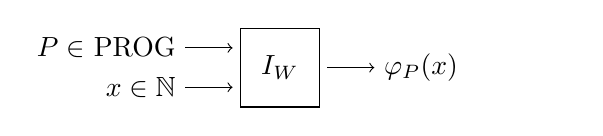
\begin{tikzpicture}
	
	\draw[->] (2.3,1.75) node[left]{$P\in\ $PROG} -- (2.9,1.75);
	\draw[->] (2.3,1.25) node[left]{$x\in \mathbb{N}$} -- (2.9,1.25);
	\draw (3,2) rectangle (4,1);
	\node at (3.5,1.5) {$I_W$};
	\draw[->] (4.1,1.5) -- (4.7,1.5)
	node [right] {$\varphi_P(x)$};
	\node[right] at (4.7,1.5) {$\phantom{\varphi_n(x)=\varphi_P(x)}$};
	
\end{tikzpicture}
\end{center}

Notiamo come l'interprete non crei dei prodotti intermedi, ma si limita a eseguire $P$ sull'input $x$.\\

Due problemi principali: 
\begin{enumerate}
	\item Il primo riguarda il tipo di input della macchina $\while$ in quanto questa non sa leggere il programma $P$ (listato di istruzioni $\ram$), sa leggere solo numeri. Dobbiamo modificare $I_W$ in modo che non passi più $P$ ma la sua codifica $cod(P) = n \in \mathbb{N}$. Questo restituisce la semantica del programma codificato con $n$, che è $P$, quindi $\varphi_n (x) ) \varphi_P (x)$
	\item Il secondo problema riguarda la quantità di dati in input alla macchina $\while$: questa legge l'input da un singolo registro, mentre qui ne stiamo passando due. Bisogna modificare $I_W$, condensando l'input tramite la funzione coppia di Cantor, che diventa $\langle x,n \rangle$
\end{enumerate}
Quindi
\begin{center}
	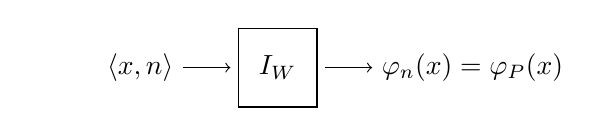
\begin{tikzpicture}
	
	\draw[->] (2.3,1.5) node[left]{$\langle x,n \rangle$} -- (2.9,1.5);
	\node[left] at (2.3,1.5) {$\phantom{cod(P)=n}$};
	\draw (3,2) rectangle (4,1);
	\node at (3.5,1.5) {$I_W$};
	\draw[->] (4.1,1.5) -- (4.7,1.5)
	node [right] {$\varphi_n(x)=\varphi_P(x)$};
	
\end{tikzpicture}
\end{center}

La semantica di $I_W$ diventa
$$ \forall x,n \in \mathbb{N} \;\;\;\; \Psi_{I_W} \left(\langle x,n \rangle \right) = \varphi_n (x) = \varphi_P (x) $$

Similmente a prima, useremo per comodità il linguaggio \textbf{macro-$\while$}, che include alcune macro comode nella scrittura di $I_W$. Viene modificata solo la sintassi e di conseguenza non la potenza del linguaggio.\\

Le \textbf{macro} utilizzate sono: 
\begin{itemize}
	\item $x_k := x_j + x_s$
	\item $x_k := \langle x_j, x_s \rangle$
	\item $x_k := \langle x_1, \dots, x_n \rangle$
	\item $x_k := \proj(x_j, x_s)$, proiezione, estrae l'elemento $x_j$-esimo dalla lista codificata in $x_s$
	\item $x_k := \incr (x_j, x_s)$, incremento, codifica la lista $x_s$ con l'elemento in posizione $x_j$-esima aumentato di 1
	\item $x_k := \decr(x_j, x_s)$, decremento, codifica la lista $x_s$ con l'elemento in posizione $x_j$-esima diminuito di 1
	\item $x_k := \sin (x_j)$
	\item $x_k := \des (x_j)$
	\item Costrutto \texttt{If} \dots \texttt{then} \dots \texttt{else}
\end{itemize}

\subsubsection{Stato della macchina $\ram$ nell'interprete}

Risolto il problema dell'input di un interprete scritto in linguaggio $\while$ per i programmi $\ram$, ora vogliamo scrivere questo interprete. In sintesi, l'interprete esegue una dopo l'altra le istruzioni $\ram$ del programma $P$ e restituisce il risultato $\varphi_P (x)$ (da notare che restituisce il risultato, non un eseguibile).\\

L'interprete ricostruisce virtualmente tutto ciò che gli serve per gestire il programma. Nel caso di $I_W$ deve ricostruire l'ambiente di una macchina $\ram$. Quello che faremo sarà ricreare il programma $P$, il Program Counter $L$ e i registri $R_0, R_1, \dots$, dentro le variabili messe a disposizione dalla macchina $\while$.\\

Primo problema: i programmi $\ram$ possono utilizzare infiniti registri, mentre i programmi $\while$ ne hanno solo 21. \textit{Ma $P$ usa veramente un numero infinito di registri?}

In realtà no; se $cod(P) = n$ allora $P$ non userà mai registri $R_j$ con $j > n$. Il programma $P$ userà sempre un numero finito di registri il cui contenuto può essere racchiuso in una lista $a_0, \dots, a_n$. La soluzione consiste nel raggruppare tutti i valori dei registri tramite Cantor $\langle a_0, \dots, a_n \rangle$ e salvarne la codifica in un unica variabile. Useremo due registri in più per comodità (possono essere utili, you never know).\\

L'interprete $I_W$ salva lo stato della macchina $\ram$ nel seguente modo (con $I_W (\langle x,n\rangle) = \varphi_n (x)$)
\begin{itemize}
	\item $x_0 \leftarrow \langle R_0, \dots, R_{n+2} \rangle$: stato della memoria della macchina $\ram$
	\item $x_1 \leftarrow L$: Program Counter
	\item $x_2 \leftarrow x$: dato su cui lavora $P$
	\item $x_3 \leftarrow n$: "listato" del programma $P$
	\item $x_4$: codice dell'istruzione da eseguire, prelevata da $x_3$ grazie a $x_1$
\end{itemize}

%P39


\end{document}
